
%(BEGIN_QUESTION)
% Copyright 2007, Tony R. Kuphaldt, released under the Creative Commons Attribution License (v 1.0)
% This means you may do almost anything with this work of mine, so long as you give me proper credit

Examine this process trend, showing the response of the process variable to a 10\% up-and-down step change in the controller output (placed in manual mode):

$$\includegraphics[width=15.5cm]{i01729x01.eps}$$

What characteristics of the process (and its related instrumentation) can you discern from this trend?  Based on this information, hypothesize how you think the controller should be tuned to respond.  In other words, how aggressive should the controller's P, I, and D terms be relative to each other?

\vskip 20pt \vbox{\hrule \hbox{\strut \vrule{} {\bf Suggestions for Socratic discussion} \vrule} \hrule}

\begin{itemize}
\item{} The possibility exists that this process is not really dominated by first-order lag at all, but rather the transmitter is heavily damped by an aggressive filtering constant.  How would the process be affected by the recommended controller tuning if in fact the first-order lag characteristic were entirely due to transmitter filtering and not the process?
\item{} The possibility exists that this process is not really dominated by first-order lag at all, but rather the control valve is slow to respond to sudden changes in controller output.  How would the process be effected by the recommended controller tuning if in fact the first-order lag characteristic were entirely due to valve lag and not the process?
\item{} Describe a diagnostic test by which you could determine whether this first-order lag is really part of the process, or is due to transmitter damping, or is due to control valve slowness.
\end{itemize}

\underbar{file i01729}
%(END_QUESTION)





%(BEGIN_ANSWER)

This is a self-regulating process dominated by first-order lag and no discernible dead time.  As such, it should be easy to control, tolerating aggressive proportional and derivative action, but requiring little integral action due to the aggressive proportional action.

%(END_ANSWER)





%(BEGIN_NOTES)

Derivative action tends to cancel first-order lag, but derivative action alone cannot maintain a process at setpoint.  Thus, proportional action is also required for robust control.  Integral action should be just enough to overcome offset in a reasonable time.  Too much integral action, and a first-order lag process will oscillate.

%INDEX% Control, PID tuning: predicting PID requirements based on open-loop response

%(END_NOTES)


